\documentclass{jlreq}

\usepackage{bm}
\usepackage{fancyhdr}
\usepackage{float}
\usepackage{graphicx}

\pagestyle{fancy}
\fancyhf{}
\fancyhead[R]{\thepage}

\renewcommand\thesubsection{(\alph{subsection})}

\title{言語処理プログラミング 課題1}
\author{22122502 川口 栄宗}
\date{提出日: \today}

\begin{document}

\maketitle
\clearpage

\section{作成したプログラムの設計情報}

\subsection{全体構成}
モジュールの関係を図\ref{fig:module_map}に示す.

\begin{figure}[H]
  \centering
  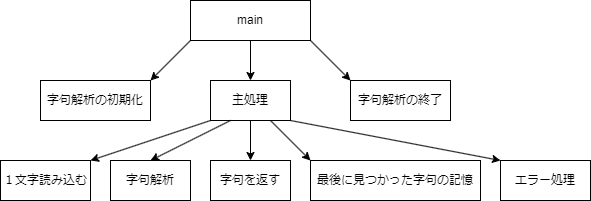
\includegraphics[width=\textwidth]{assets/lpp01_module.png}
  \caption{モジュール構成図}
  \label{fig:module_map}
\end{figure}

\subsection{各モジュールごとの構成}
モジュール間で共通した変数を以下に示す.
\begin{table}[H]
  \centering
  \caption{モジュール間で共通して用いる変数}
  \begin{tabular}{|c|c|c|}
    \hline
    変数名 & 型    & 説明                                                    \\  \hline
    cbuf   & int   & ファイルから読み込んだ次の1文字の文字コードを格納する. \\ \hline
    fp     & FILE* & ファイルポインタ                                        \\ \hline
  \end{tabular}
\end{table}

\subsubsection{字句解析の初期化}
init\_scan関数内で初期化を行う.初期化処理では,mpplファイルの読み込み,ファイルポインタを用いた1文字の読み込み,
linenumへの0の代入,num\_attributeを-1にする処理を施す.

\subsubsection{主処理}
解析対象の字句に対してfgetc(fp)でファイルの文字を1文字ずつ読み込み,先頭の文字などで場合分けを行うことで
字句解析をscan関数内で行っている.scanが-1を返したときに,main関数内での解析処理は終わり,end\_scan関数を呼び出して主な処理は終了する.
エラーが発生した場合は戻り値としてS\_ERROR(-1)を返すとともに,error関数で標準エラー出力にエラーメッセージを表示して字句解析を終了させる.

\subsubsection{字句解析の終了}
end\_scan関数内で行う.ここでは,mpplファイルを閉じる処理のみが実行される.

\subsection{各関数の外部(入出力)使用}

\subsubsection{init\_scan}
\begin{description}
  \item[機能] スキャナーを初期化する
  \item[引数] ファイル名(char型へのポインタ)
  \item[戻り値] 成功の場合は0,ファイルオープンに失敗した場合は-1
\end{description}

\subsubsection{end\_scan}
\begin{description}
  \item[機能] ファイルを閉じて,スキャナーを終了する
  \item[引数] なし
  \item[戻り値] なし
\end{description}

\subsubsection{scan}
\begin{description}
  \item[機能] 字句解析を行う
  \item[引数] なし
  \item[戻り値] 字句解析に成功した場合は字句のコード(int型),コメントや改行を検出した場合は0,字句解析に失敗した場合はS\_ERROR(-1)
\end{description}

\subsubsection{push\_char}
\begin{description}
  \item[機能] スキャナーを初期化する
  \item[引数] ファイル名(char型へのポインタ)
  \item[戻り値] 成功の場合は0,ファイルオープンに失敗した場合は-1
\end{description}

\subsubsection{pop\_char}
\begin{description}
  \item[機能] スキャナーを終了する
  \item[引数] なし
  \item[戻り値] なし
\end{description}

\subsubsection{clear\_string\_attr}
\begin{description}
  \item[機能] スキャナーを初期化する
  \item[引数] ファイル名(char型へのポインタ)
  \item[戻り値] 成功の場合は0,ファイルオープンに失敗した場合は-1
\end{description}

\subsubsection{is\_keyword}
\begin{description}
  \item[機能] スキャナーを初期化する
  \item[引数] ファイル名(char型へのポインタ)
  \item[戻り値] 成功の場合は0,ファイルオープンに失敗した場合は-1
\end{description}

\subsubsection{get\_linenum}
\begin{description}
  \item[機能] スキャナーを初期化する
  \item[引数] ファイル名(char型へのポインタ)
  \item[戻り値] 成功の場合は0,ファイルオープンに失敗した場合は-1
\end{description}

\subsubsection{skip\_blank}
\begin{description}
  \item[機能] スキャナーを初期化する
  \item[引数] ファイル名(char型へのポインタ)
  \item[戻り値] 成功の場合は0,ファイルオープンに失敗した場合は-1
\end{description}

\subsubsection{skip\_bracket\_comment}
\begin{description}
  \item[機能] スキャナーを初期化する
  \item[引数] ファイル名(char型へのポインタ)
  \item[戻り値] 成功の場合は0,ファイルオープンに失敗した場合は-1
\end{description}

\subsubsection{skip\_slash\_comment}
\begin{description}
  \item[機能] スキャナーを初期化する
  \item[引数] ファイル名(char型へのポインタ)
  \item[戻り値] 成功の場合は0,ファイルオープンに失敗した場合は-1
\end{description}

\subsubsection{error}
\begin{description}
  \item[機能] スキャナーを初期化する
  \item[引数] ファイル名(char型へのポインタ)
  \item[戻り値] 成功の場合は0,ファイルオープンに失敗した場合は-1
\end{description}


\section{テスト情報}

\subsection{テストデータ}
\subsection{テスト結果}
\subsection{テストデータの十分性}

\section{課題のスケジュールと実際の進捗状況}

\subsection{事前計画}
\subsection{実際の進捗状況}
\subsection{当初の事前計画と実際の進捗との差の原因}

\end{document}